\section{Modelo de datos}
	\subsection{Modelo de base de datos}
		\begin{figure}[htbp!]
			\centering
				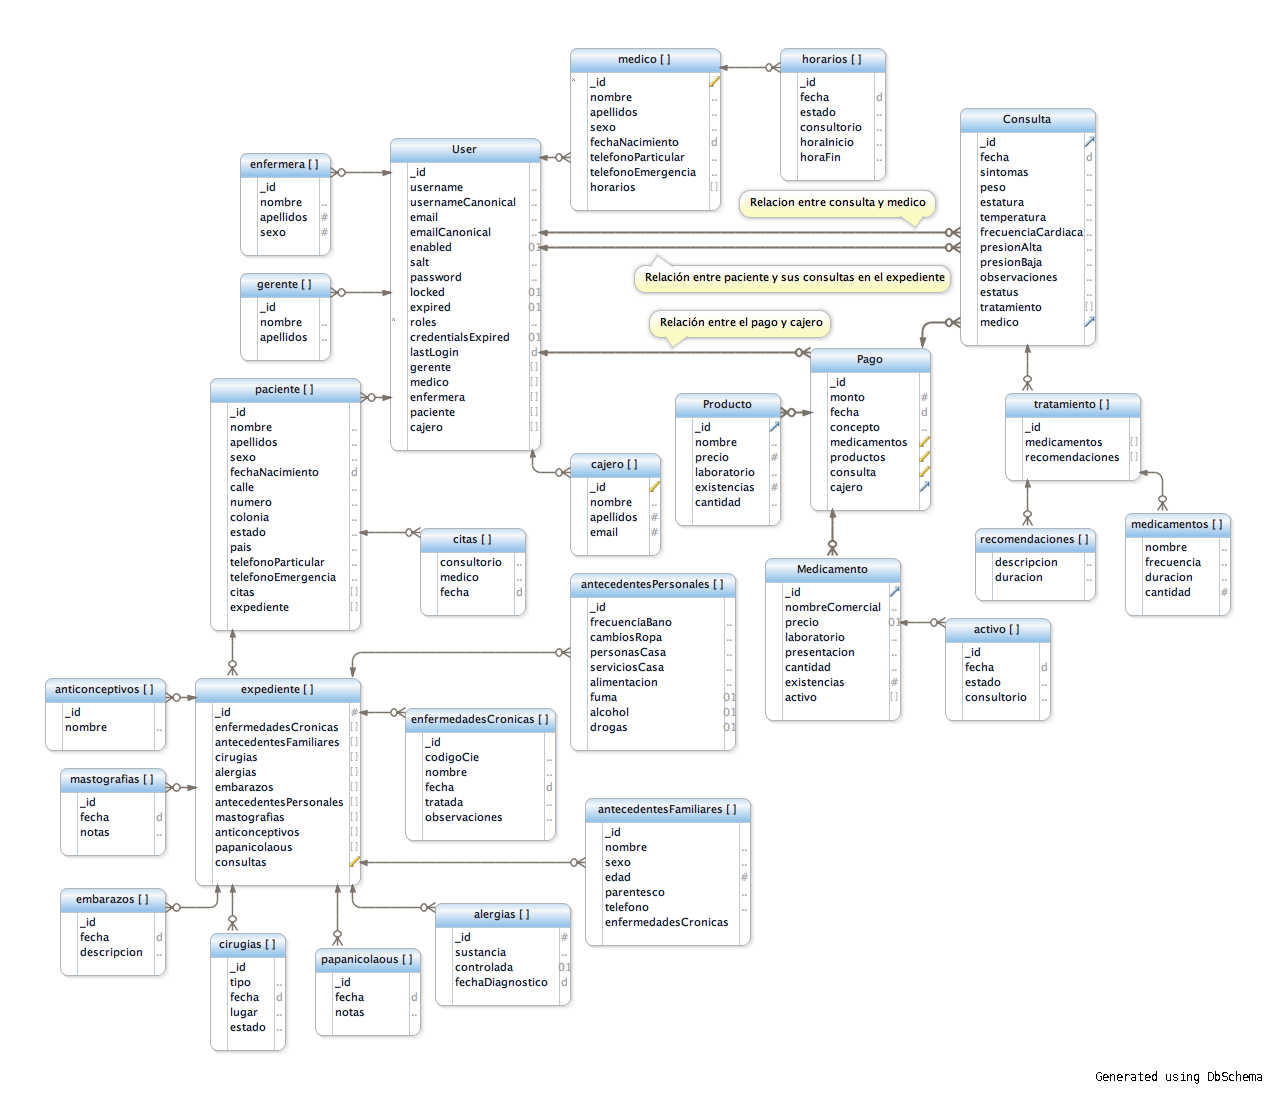
\includegraphics[width=1\textwidth]{images/modeloDatos}
			\caption{Modelo de base de datos}
		\end{figure}
		\newpage
	\subsection{Modelo entidad-relación}
	\newpage
	\subsection{Diccionario de datos}
	\begin{table}[htb]
	\centering
	\begin{tabular}{| p{3.5cm}| p{3.0cm} | p{9.8cm} |}
	\hline
	\multicolumn{3}{|c|}{Colección : User} \\
	\hline
	Campo & Tipo &  Descripción\\ \hline
	\_id & ObjectId & Identificador único de mongodb para el usuario \\ \hline
	username & String & Nombre completo del usuario.\\ \hline
	usernameCanonical & String & Copia del nombre completo del usuario.\\ \hline
	email & String & Email del usuario.\\ \hline
	emailCanonical & String & Copia del email original del usuario.\\ \hline
	enabled & Boolean & Atributo booleano para determinar si el usuario esta habilitado o no.\\ \hline
	salt & String & Número de dígitos aleatorios que se le agregan al hash del password para hacer más segura la contraseña \\ \hline
	password & String & Hash de la contraseña del usuario.\\ \hline
	locked & Boolean & Atributo booleano para determinar si el usuario esta bloqueado o no.\\ \hline
	expired & Boolean & Atributo booleano para determinar si la cuenta del usuario ha expirado. \\ \hline
	roles & Array & Arreglo de roles que tiene el usuario. \\ \hline
	credentialsExpired & Boolean & Atributo booleano para determinar si las credenciales del usuario han expirado. \\ \hline
	lastLogin & Date & Fecha del último login del usuario en el sistema. \\ \hline
	gerente & EmbeddedDocument & Documento embebido para almacenar la información del usuario de tipo gerente \\ \hline
	medico & EmbeddedDocument & Documento embebido para almacenar la información del usuario de tipo \\ \hline
	enfermera & EmbeddedDocument & Documento embebido para almacenar la información del usuario de tipo enfermera \\ \hline
	paciente & EmbeddedDocument & Documento embebido para almacenar la información del usuario de tipo paciente \\ \hline
	cajero & EmbeddedDocument & Documento embebido para almacenar la información del usuario de tipo cajero \\ \hline
	\end{tabular}
	\caption{Tabla de la colección del User.}
	\label{tabla:diccionarioDatos}
	\end{table}
	%=========================================================
	\begin{table}[htb]
	\centering
	\begin{tabular}{| p{3.5cm}| p{3.0cm} | p{9.8cm} |}
	\hline
	\multicolumn{3}{|c|}{Documento embebido : enfermera} \\
	\hline
	Campo & Tipo &  Descripción\\ \hline
	\_id & ObjectId & Identificador único de mongodb para la enfermera \\ \hline
	nombre & String & Nombre(s) de la enfemera.\\ \hline
	apellidos & String & Apellidos de la enfermera.\\ \hline
	sexo & String & Condición orgánica que para distinguir de hombres y mujeres .\\ \hline
	\end{tabular}
	\caption{Tabla del documento embebido de la enfermera .}
	\label{tabla:diccionarioDatos}
	\end{table}
	%=========================================================
	\begin{table}[htb]
	\centering
	\begin{tabular}{| p{3.5cm}| p{3.0cm} | p{9.8cm} |}
	\hline
	\multicolumn{3}{|c|}{Documento embebido : gerente} \\
	\hline
	Campo & Tipo &  Descripción\\ \hline
	\_id & ObjectId & Identificador único de mongodb para el gerente \\ \hline
	nombre & String & Nombre(s) del gerente.\\ \hline
	apellidos & String & Apellidos del gerente.\\ \hline
	\end{tabular}
	\caption{Tabla del documento embebido del gerente .}
	\label{tabla:diccionarioDatos}
	\end{table}
	%=========================================================
	\begin{table}[htb]
	\centering
	\begin{tabular}{| p{3.5cm}| p{3.0cm} | p{9.8cm} |}
	\hline
	\multicolumn{3}{|c|}{Documento embebido : cajero} \\
	\hline
	Campo & Tipo &  Descripción\\ \hline
	\_id & ObjectId & Identificador único de mongodb para el cajero \\ \hline
	nombre & String & Nombre(s) del cajero.\\ \hline
	apellidos & String & Apellidos del cajero.\\ \hline
	\end{tabular}
	\caption{Tabla del documento embebido del cajero .}
	\label{tabla:diccionarioDatos}
	\end{table}
	%=========================================================
	\begin{table}[htb]
	\centering
	\begin{tabular}{| p{3.5cm}| p{3.0cm} | p{9.8cm} |}
	\hline
	\multicolumn{3}{|c|}{Documento embebido : medico} \\
	\hline
	Campo & Tipo &  Descripción\\ \hline
	\_id & ObjectId & Identificador único de mongodb para el médico \\ \hline
	nombre & String & Nombre(s) del médico.\\ \hline
	apellidos & String & Apellidos del médico.\\ \hline
	sexo & String & Condición orgánica que para distinguir de hombres y mujeres .\\ \hline
	fechaNacimiento & Date &  Fecha de nacimiento del médico.\\ \hline
	telefonoParticular & String & Telefono particular para contactar al médico.\\ \hline
	telefonoEmergencia & String & Telefono de emergencia para contactar al médico.\\ \hline
	horarios & EmbeddedDocument(s) &  Documento(s) embebido(s) para almacenar la información pertinente al horario de servicio del médico.\\ \hline

	\end{tabular}
	\caption{Tabla del documento embebido del médico .}
	\label{tabla:diccionarioDatos}
	\end{table}
	%=========================================================
	\begin{table}[htb]
	\centering
	\begin{tabular}{| p{3.5cm}| p{3.0cm} | p{9.8cm} |}
	\hline
	\multicolumn{3}{|c|}{Documento embebido : paciente} \\
	\hline
	Campo & Tipo &  Descripción\\ \hline
	\_id & ObjectId & Identificador único de mongodb para el paciente \\ \hline
	nombre & String & Nombre(s) del médico.\\ \hline
	apellidos & String & Apellidos del médico.\\ \hline
	sexo & String & Condición orgánica que para distinguir de hombres y mujeres .\\ \hline
	fechaNacimiento & Date &  Fecha de nacimiento del paciente.\\ \hline
	calle & String & Calle del \textit{domicilio donde reside }el paciente actualmente\\ \hline
	numero & String & Telefono de emergencia para contactar al médico.\\ \hline
	citas & EmbeddedDocument(s) &  Documento(s) embebido(s) para almacenar la información pertinente a las citas del paciente.\\ \hline

	\end{tabular}
	\caption{Tabla del documento embebido del paciente .}
	\label{tabla:diccionarioDatos}
	\end{table}
	%=========================================================

	\newpage

\section{Modelo de acceso de datos}


